\documentclass[11pt,a4paper]{article}

\usepackage[T1]{fontenc}
\usepackage[utf8]{inputenc}
\usepackage{lmodern}
\usepackage{amsmath}
\usepackage[a4paper,margin=24mm]{geometry}
\usepackage{booktabs}
\usepackage{graphicx}
\usepackage{float}
\usepackage{caption}
\usepackage{enumitem}
\usepackage[hidelinks]{hyperref}
\Urlmuskip=0mu plus 1mu\relax
\makeatletter
\def\UrlBreaks{\do\/\do\-\do\.\do\:\do\=\do\?\do\&\do\_%
  \do\a\do\b\do\c\do\d\do\e\do\f\do\g\do\h\do\i\do\j\do\k\do\l\do\m%
  \do\n\do\o\do\p\do\q\do\r\do\s\do\t\do\u\do\v\do\w\do\x\do\y\do\z%
  \do\0\do\1\do\2\do\3\do\4\do\5\do\6\do\7\do\8\do\9}
\makeatother
\captionsetup{font=small,labelfont=bf,skip=6pt}
\setlist{nosep,leftmargin=1.4em}
\graphicspath{{../progress-report/assets/}}
\setlength{\parskip}{0.4\baselineskip}
\setlength{\parindent}{0pt}
\frenchspacing

\title{\vspace{-8mm}BeSecured: a local cybersecurity risk scanner\\[3pt]
  \large P12 final report}
\author{Mohammedreda El Aroui (project manager), Sidi Hamadi,\\
  Philemon Vittet, Abdelrahmn Dahy}
\date{June 2026}

\begin{document}
\maketitle

BeSecured looks at the security settings of a personal computer and turns them
into a score out of 100, with a short list of things to fix. It is meant for
people who are not security experts. This is the final report for project P12,
Personal Cybersecurity Risk Scanner.

\section{Existing tools and where BeSecured fits}

The tools a person can actually reach today fall into a few groups, and each one
leaves the same gap. Consumer antivirus suites, such as Microsoft Defender,
Norton, Bitdefender and McAfee, are built to catch malware in real time and
mostly show their own features as on or off. Only McAfee gives a number, and that
number rates how fully you turned on McAfee's features and your identity
exposure, not how the machine is configured. The operating system gets closest to
a posture panel. Windows Security shows each area in green, amber or red, but it
is Windows only and never adds up to a single score, macOS has no such dashboard,
and on Linux the same signals are spread across separate command-line tools.

Two groups go deeper, in opposite directions. Host hardening auditors, such as
Lynis, CIS-CAT and OpenSCAP, do check configuration rather than malware, and
CIS-CAT even gives a score out of 100. They are made for system administrators
and auditors, though: a command line or root access or a Java app, reports keyed
to benchmark rule numbers, and some checks behind a paid membership. Network and
vulnerability scanners, such as Nmap, OpenVAS, Nessus and Qualys, are more
powerful still, but they probe the network for known vulnerabilities across many
machines, can be intrusive, need authorisation, and assume an expert at the
keyboard. They answer what is reachable on the network, not whether one personal
machine is set up safely. The products that do hand out a security score, such as
Microsoft Secure Score, SecurityScorecard and Bitsight, rate a company's cloud
tenant or its whole internet footprint, and the one consumer checkup, from
Google, only looks at the Google account.

The gap they all leave is the same: a local, read-only check that gives a
non-technical person a single score and plain-language fixes for their own
computer, across Windows, macOS and Linux, with no account, no cloud and no
network probing. Each piece exists somewhere, but no single tool puts them
together for a home user. BeSecured aims at that gap and nothing wider. It is
shallow next to a benchmark auditor or a vulnerability scanner, since it reads a
handful of settings rather than a full benchmark, and a professional would still
use the heavier tools. The contribution is fit, not depth. The direction is
supported by work on usable security: a NIST study on security fatigue found that
ordinary users are worn down by the sheer number of security decisions they face,
and a comparison of expert and non-expert habits found that non-experts often
fall back on advice that does little to protect them. Both point to the same need,
prioritised guidance in plain language for individuals, rather than one more
technical report.

\begin{table}[h]
\centering\footnotesize
\setlength{\tabcolsep}{4pt}
\begin{tabular}{@{}p{0.19\linewidth}p{0.27\linewidth}p{0.12\linewidth}p{0.19\linewidth}p{0.11\linewidth}@{}}
\toprule
Tool group & Mainly checks & For whom & Local, non-intrusive & All three systems \\
\midrule
Consumer antivirus (Defender, Norton, Bitdefender, McAfee) & Malware in real time, features on or off; only McAfee shows a number, for its own features & Home users & Local agent, but cloud-linked and account-based, mostly paid & Mixed; Defender itself is Windows only \\
Built-in OS security (Windows Security, macOS Gatekeeper and FileVault, Linux ufw) & Per-area status, no overall score; macOS has no dashboard, Linux is command line & Each platform's users & Local and read-only & No, one OS each \\
Hardening auditors (Lynis, CIS-CAT, OpenSCAP) & Configuration against a benchmark; CIS-CAT scores 1 to 100, output keyed to rule numbers & Sysadmins and auditors & Local, but command line or root or Java, some checks paid & Mixed, none covers all three simply \\
Vulnerability and network scanners (Nmap, OpenVAS, Nessus, Qualys) & Network and known-vulnerability discovery across many hosts & Security professionals & No, probes the network, can be intrusive, often costly & Scans any OS, but heavy to run \\
Enterprise scores and ratings (Secure Score, SecurityScorecard, Bitsight) & A score, but for a cloud tenant or a whole organisation & Enterprise and risk teams & Cloud or SaaS, account-based & No, not a device check \\
\midrule
BeSecured (this project) & One 0 to 100 score for a personal machine, with plain-language fixes; modest depth & Non-technical individuals & Yes, fully local, standard library only, nothing leaves the machine & Yes, Windows, macOS and Linux \\
\bottomrule
\end{tabular}
\caption{Existing tools by group, and where BeSecured sits. BeSecured is the only
row that is local, plain-language and cross-platform for a non-expert, and also
the shallowest.}
\end{table}

\section{The plan and the objectives}

BeSecured is a ten-week project for a team of four, run as weekly sprints. The
brief asks for a lightweight tool that scans a personal machine for common
weaknesses, turns the result into a clear risk score, and tells a non-technical
user what to fix first. It is not a pentest tool and not an antivirus. The point
is a readable picture of local risk, not an audit.

The main objectives, taken from the charter and the project plan, were:

\begin{itemize}
\item run a local scan from a single action, with no setup for the user;
\item produce a cybersecurity risk score from 0 to 100 after each scan;
\item list the detected issues by severity, each with a plain-language
  explanation and concrete fix steps;
\item export the result as a report;
\item keep everything local: no account, nothing stored or sent off the machine;
\item cover the three desktop systems, Windows, macOS and Linux.
\end{itemize}

The plan split this into ten one-week sprints: charter, planning and design, then
the scanner, the scoring engine, the interface and report export, an optional AI
step, testing, and final delivery. Work was prioritised with MoSCoW, tracked
against a risk register, and reviewed each week. Two items were flagged from the
start as the first to drop if time ran short: a React and Tailwind dashboard, and
an optional large language model step to phrase the explanations. Both were
dropped.

\section{What the tool does now}

We started from a PowerShell script that only ran on Windows. BeSecured is now a
Python package with no third-party dependency in the scan engine. A single entry
point runs the checks that apply to any system, then the ones specific to the
current operating system, collects the findings, and computes the score.

\begin{table}[h]
\centering\small
\begin{tabular}{@{}ll@{}}
\toprule
Module & Responsibility \\
\midrule
\texttt{scanner.py} & Entry point: runs the checks, dispatches by OS, builds the result. \\
\texttt{checks/common.py} & System info, privileges, listening ports. \\
\texttt{checks/windows.py} & Firewall, Defender, updates, users, policy, shares, startup, UAC, BitLocker. \\
\texttt{checks/macos.py} & Firewall, FileVault, Gatekeeper, SIP, XProtect, sharing, login items. \\
\texttt{checks/linux.py} & Firewall, updates, LUKS, users, password rules, shares, startup, antivirus. \\
\texttt{models.py} & Finding and result data, with a stable JSON shape. \\
\texttt{scoring.py} & Score, grade, per-category and per-finding impact. \\
\texttt{report.py} & HTML and JSON export. \\
\texttt{app.py}, \texttt{ui/} & Native window and local development server. \\
\bottomrule
\end{tabular}
\end{table}

Each operating system has its own module, but the categories line up so the score
reads the same way everywhere. The scan reads ten areas.

\begin{table}[h]
\centering\small
\begin{tabular}{@{}lll@{}}
\toprule
Area & What it reads & Platforms \\
\midrule
Open ports & Listening TCP ports and risky services (RDP, SMB, SSH, VNC) & all \\
Firewall & Local firewall state and profiles & all \\
Updates & Freshness of system and software updates & all \\
Accounts & Administrators, guest access, accounts without a password & all \\
Password policy & Minimum length and expiry, where readable & Win, Linux \\
Shared folders & SMB, NFS or non-standard system shares & all \\
Startup programs & Startup entries, with temporary paths flagged & all \\
Protection & Antivirus or native protection and signature freshness & all \\
Disk encryption & BitLocker, FileVault or LUKS state & all \\
Hardening & UAC on Windows, Gatekeeper and SIP on macOS & Win, macOS \\
\bottomrule
\end{tabular}
\end{table}

The parsing of each check is defensive on purpose. System tools differ a lot
between machines and versions, so a parser that assumes one fixed format breaks
easily. A malformed or missing output becomes a skipped check with a short note,
not a crash, and each check is isolated so one failure never aborts the scan.

\subsection*{Scoring}

A check ends as OK, a warning, or critical; a few are marked info or skipped.
Only the first three move the score. A warning costs 2 points, a critical one
costs 5, and the final score is 100 minus the share of points lost.
\[
\text{score} = 100 - \operatorname{round}\!\left(\frac{\text{points lost}}{\text{points possible}} \times 100\right)
\]
Points possible is the number of scored checks times 5, the most a scan could
lose. A skipped check, for example one that needs administrator rights we do not have,
is shown as skipped and never counted as a pass. We would rather show a gap than
hide it. The grade follows the score: A from 90, B from 75, C from 60, D from 40,
F below.

\subsection*{The interface}

The interface opens in its own window through pywebview, the webview built into
the operating system, so there is no browser, no address bar and no open port
when the app runs natively. The original local web server is kept as a
development harness and a fallback. The interface has five screens: a home screen
to start the scan and see what gets checked, an overview with the score, a list
of categories, a list of issues to fix, and a report screen. Each finding states
what was seen, why it matters, and the steps to fix it
(Figures~\ref{fig:home}, \ref{fig:issues} and~\ref{fig:overview}).

\begin{figure}[H]
\centering
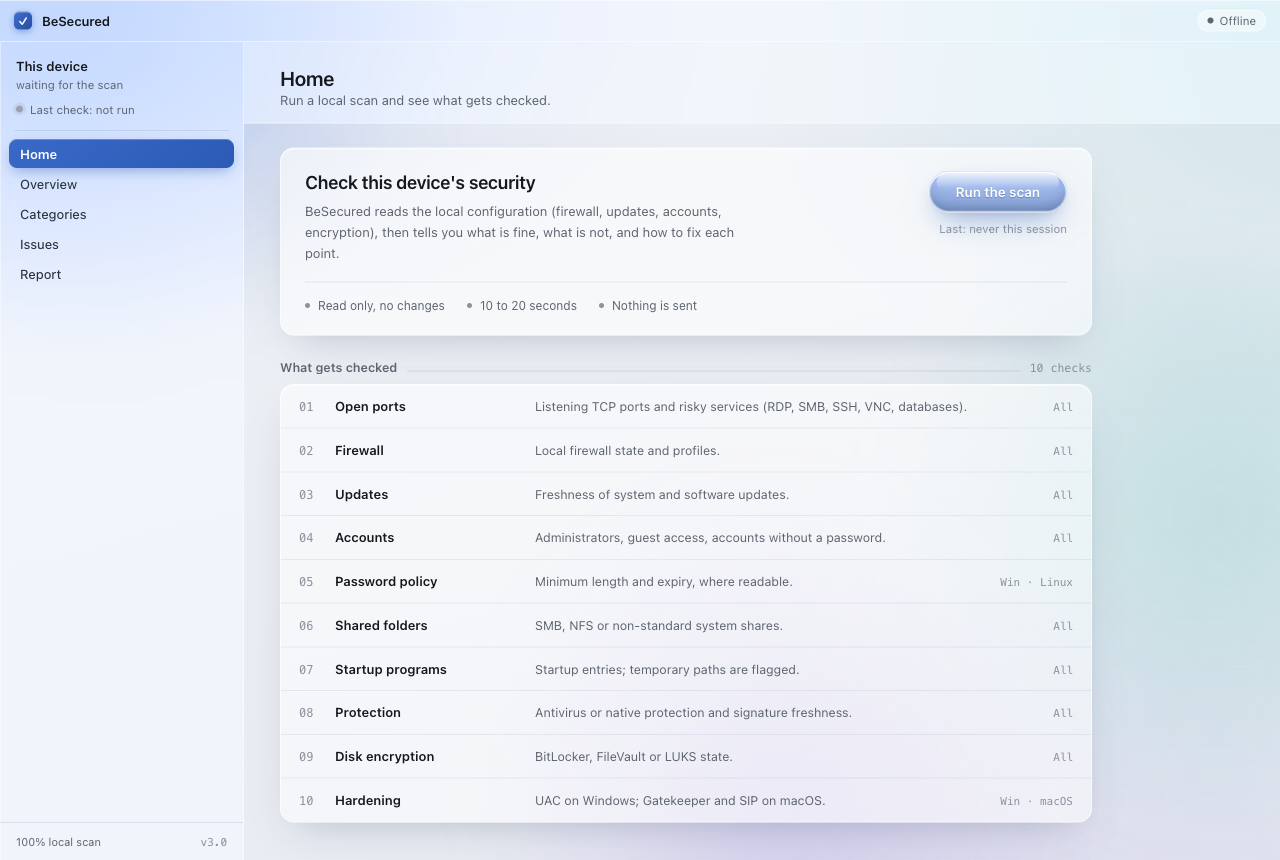
\includegraphics[width=0.80\linewidth]{ui-home.png}
\caption{Home screen: one action to start, and the list of what the scan reads.
The window opens in its own frame, without a browser address bar.}
\label{fig:home}
\end{figure}

The colours and the motion are deliberate. Every text colour clears the WCAG AA
contrast ratio of 4.5 to 1 on white, and severity is never shown by colour alone:
each finding carries a colour, an icon and a label, because about one man in
twelve cannot tell red from green. Motion is kept to a few short transitions and
respects the system reduced-motion setting. The reasoning is written down in two
short research notes kept in the repository.

\begin{figure}[H]
\centering
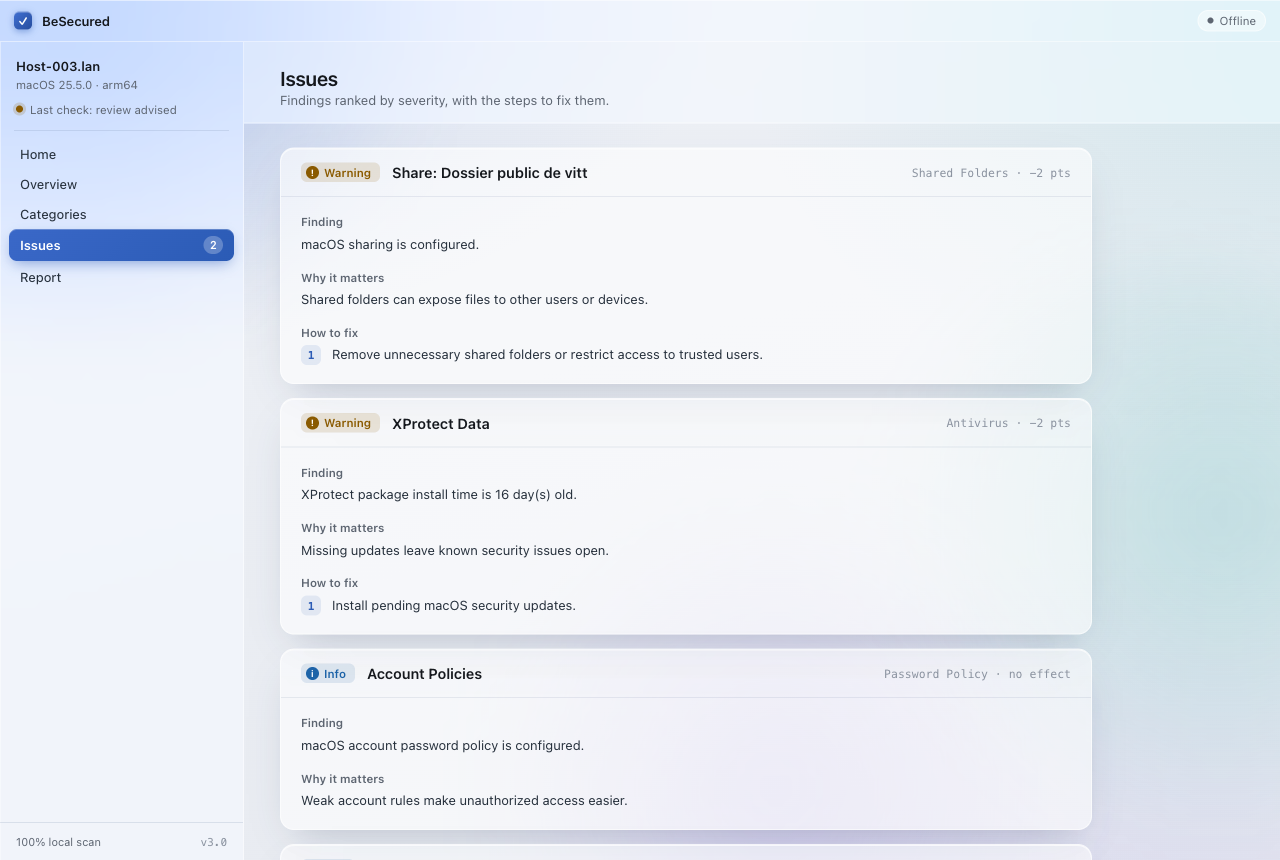
\includegraphics[width=0.80\linewidth]{ui-issues.png}
\caption{Issues, ranked by severity. Severity is shown by colour, an icon and a
label at once, so it stays readable for colour-blind users.}
\label{fig:issues}
\end{figure}

\begin{figure}[H]
\centering
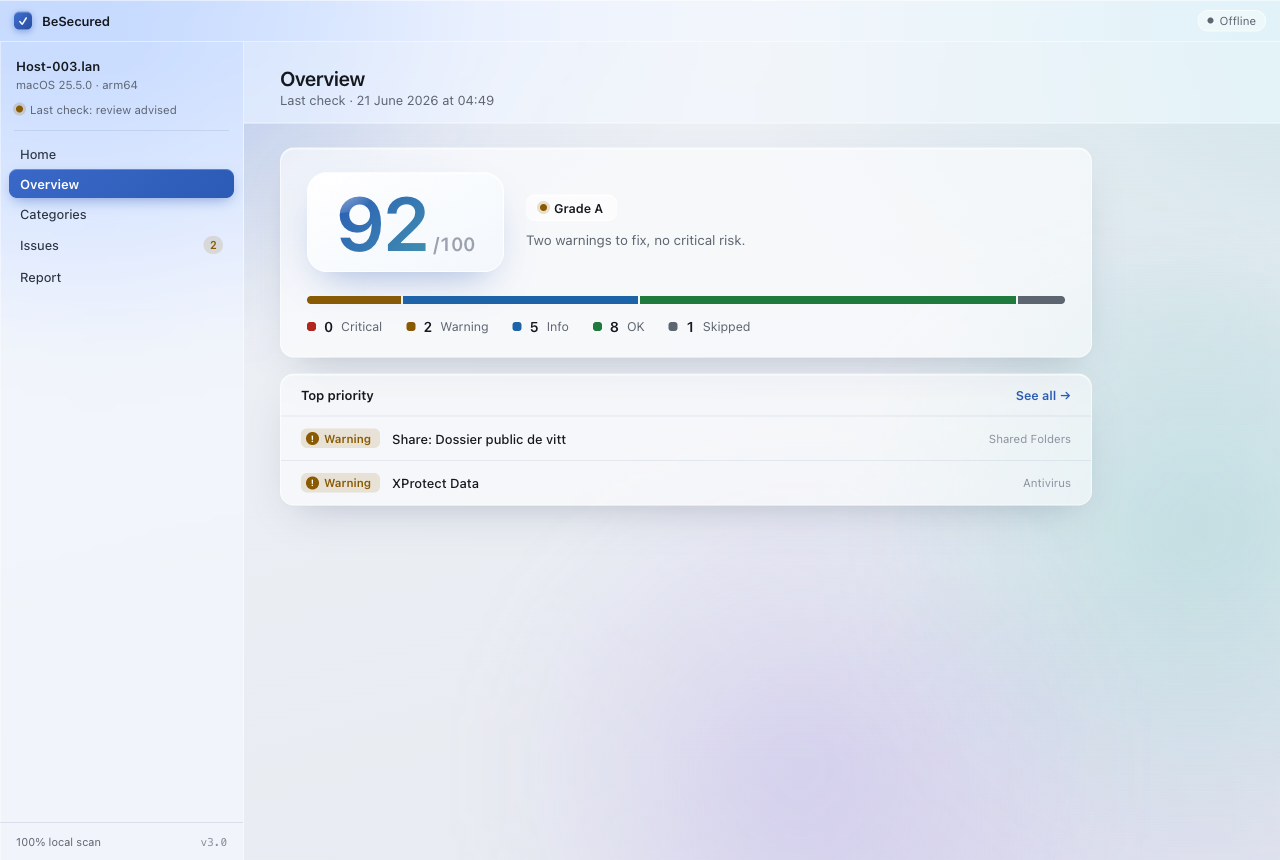
\includegraphics[width=0.80\linewidth]{ui-overview.png}
\caption{Overview after a scan: the score out of 100, the grade, and the
breakdown by status. This run scored 92, grade A, with two warnings and no
critical issue.}
\label{fig:overview}
\end{figure}

\subsection*{Privacy and packaging}

Nothing leaves the machine. There is no account and no remote backend. In the
native app the interface talks to the engine through an internal bridge, with no
port open; in the development web mode it listens on 127.0.0.1. Reports are
written to a local folder, and the program refuses to write one onto a
cloud-synced path such as iCloud, OneDrive or Dropbox, so a report cannot leave
the device by accident. A test checks that the interface files hold no external
link, which keeps the promise honest as the code changes.

The app is packaged with PyInstaller into a double-click bundle,
\texttt{BeSecured.app} on macOS and \texttt{BeSecured.exe} on Windows. The macOS
build is done locally; the Windows build needs a Windows machine, because
PyInstaller does not cross-compile. The binaries are not signed, so the system
shows a one-time warning on first launch, which we document rather than pay to
remove.

\section{Objectives achieved}

The committed scope is delivered.

\begin{table}[h]
\centering\small
\begin{tabular}{@{}p{0.42\linewidth}p{0.52\linewidth}@{}}
\toprule
Objective & Result \\
\midrule
Local one-action scan & Done. CLI, native app, and web development UI. \\
Risk score 0 to 100 & Done. Every scan returns a score, a grade and the points lost. \\
Issues by severity, with explanation and fix steps & Done. Every finding carries a plain-language reason and a concrete action. \\
Report export & Done as HTML and JSON. The HTML prints to PDF. \\
Local only, nothing transmitted & Done. Local design, cloud-path guard, external-link test. \\
Windows, macOS and Linux & Done. One engine, a module per system. \\
\bottomrule
\end{tabular}
\end{table}

The optional large language model step, backlog item US10, marked Won't, was not
built. The need it addressed, plain-language explanations, is already met by the
rule-based text the engine writes for every finding.

The plan listed two success criteria
that need a study we did not run: a detection rate against a labelled set of test
vulnerabilities, and a comprehension rate from real test users. We did not
benchmark a detection percentage or run a formal user survey, so we do not claim
those figures. What we can show is stability and privacy. The project has 102
automated tests and they all pass. The suite runs with
\texttt{python -m unittest discover -s tests} and covers the parsers and checks
for each operating system, the dispatch to the right OS module, the scoring and
the grades, the HTML and JSON export, the JSON contract between the scanner and
the interface, the local scan endpoint, and a guard that the interface holds no
remote reference. The local-only promise is held up by these last tests rather
than by a claim in a document.

\section{Lessons learned}

Dropping the React, Tailwind and Chart.js stack was the right call, and not only
to save time. A tool whose whole promise is that nothing leaves the machine is
easier to trust when there is nothing to leave with. The engine has no
third-party dependency, and a single test forbids any external link in the
sensitive sources. Fewer moving parts also meant the whole thing ships as one
double-click file.

The real work was parsing real system output, not the security logic itself. The
output of tools like \texttt{ss}, \texttt{lsof}, \texttt{netstat}, PowerShell and
the various update commands changes between machines and versions. Moving from
``assume a format'' to ``an unreadable output is a skipped check, not a crash''
is most of the reason the test count grew through the project. It also set a rule
we kept: a skipped check is never counted as a pass, because hiding a gap would
mislead exactly the non-expert we built this for.

Treating the AI step as optional protected the schedule. Because the user-facing
explanation was already met with rule-based text, the optional step could be
dropped late without breaking a promise. Marking it Won't at planning time,
rather than discovering the cut under pressure in the last sprint, is what made
that painless.

Building for three systems from one codebase forced a clean split early: common
checks, then a module per OS, with categories that line up so the score means the
same thing everywhere. That structure let us test each system's parsing on its own.

\section{Further work}

With the scan engine and 102 passing tests in place, the next steps add reach
rather than new core features.

\begin{itemize}
\item Build and sign the Windows executable on a Windows machine, and sign the
  macOS bundle, to remove the first-launch warning.
\item Improve detection of third-party protection beyond the native tools.
\item Keep a local-only scan history so a user can compare results over time
  (backlog item US09, Could).
\item Add finer scoring profiles for a personal machine versus a small
  organisation.
\item Revisit local, offline explanations now that the rule-based layer is
  stable, kept on the machine to preserve the privacy promise.
\end{itemize}

\section*{Sources}
\small
\begin{enumerate}
\item B. Stanton, M. Theofanos, S. Prettyman, S. Furman. Security fatigue. IEEE
  IT Professional, 2016. \url{https://csrc.nist.gov/pubs/journal/2016/09/security-fatigue/final}
\item I. Ion, R. Reeder, S. Consolvo. ``...No one can hack my mind'': comparing
  expert and non-expert security practices. SOUPS, 2015.
  \url{https://www.usenix.org/conference/soups2015/proceedings/presentation/ion}
\item Lynis, CISOfy. \url{https://cisofy.com/lynis/}
\item CIS-CAT, Center for Internet Security. \url{https://www.cisecurity.org/cybersecurity-tools/cis-cat-pro}
\item OpenSCAP. \url{https://www.open-scap.org/}
\item Nessus, Tenable. \url{https://www.tenable.com/products/nessus}
\item Microsoft Secure Score. \url{https://learn.microsoft.com/en-us/defender-xdr/microsoft-secure-score}
\item Windows Security. \url{https://support.microsoft.com/en-us/windows/stay-protected-with-windows-security-2ae0363d-0ada-c064-8b56-6a39afb6a963}
\item Google Security Checkup. \url{https://support.google.com/accounts/answer/12629482}
\item McAfee Protection Score. \url{https://www.mcafee.com/en-us/antivirus/protection-score.html}
\end{enumerate}

\end{document}
